% Author: Izaak Neutelings (September 2021)
% Inspiration:
%   https://www.asimovinstitute.org/neural-network-zoo/
%   https://www.youtube.com/watch?v=aircAruvnKk&list=PLZHQObOWTQDNU6R1_67000Dx_ZCJB-3pi&index=1
% https://tikz.net/neural_networks/
\documentclass[border=3pt,tikz]{standalone}
\usepackage{amsmath} % for aligned
%\usepackage{amssymb} % for \mathbb
\usepackage{tikz}
%\usepackage{etoolbox} % for \ifthen
\usepackage{listofitems} % for \readlist to create arrays
\usetikzlibrary{arrows.meta} % for arrow size
\usepackage[outline]{contour} % glow around text
\contourlength{1.4pt}

\tikzset{>=latex} % for LaTeX arrow head
\usepackage{xcolor}
\colorlet{myred}{red!80!black}
\colorlet{myblue}{blue!80!black}
\colorlet{mygreen}{green!60!black}
\colorlet{myorange}{orange!70!red!60!black}
\colorlet{mydarkred}{red!60!black}
\colorlet{mydarkblue}{blue!60!black}
\colorlet{mydarkgreen}{green!50!black}
\tikzstyle{node}=[thick,circle,draw=myblue,minimum size=22,inner sep=0.5,outer sep=0.6]
\tikzstyle{node in}=[node,green!20!black,draw=mygreen!30!black,fill=mygreen!25]
\tikzstyle{node hidden}=[node,blue!20!black,draw=myblue!30!black,fill=myblue!20]
\tikzstyle{node convol}=[node,orange!20!black,draw=myorange!30!black,fill=myorange!20]
\tikzstyle{node out}=[node,red!20!black,draw=myred!30!black,fill=myred!20]
\tikzstyle{connect}=[thick,mydarkblue] %,line cap=round
\tikzstyle{connect arrow}=[-{Latex[length=4,width=3.5]},thick,mydarkblue,shorten <=0.5,shorten >=1]
\tikzset{ % node styles, numbered for easy mapping with \nstyle
  node 1/.style={node in},
  node 2/.style={node hidden},
  node 3/.style={node out},
}
\def\nstyle{int(\lay<\Nnodlen?min(2,\lay):3)} % map layer number onto 1, 2, or 3

\begin{document}


% NEURAL NETWORK with x, a, y coefficients, arrows
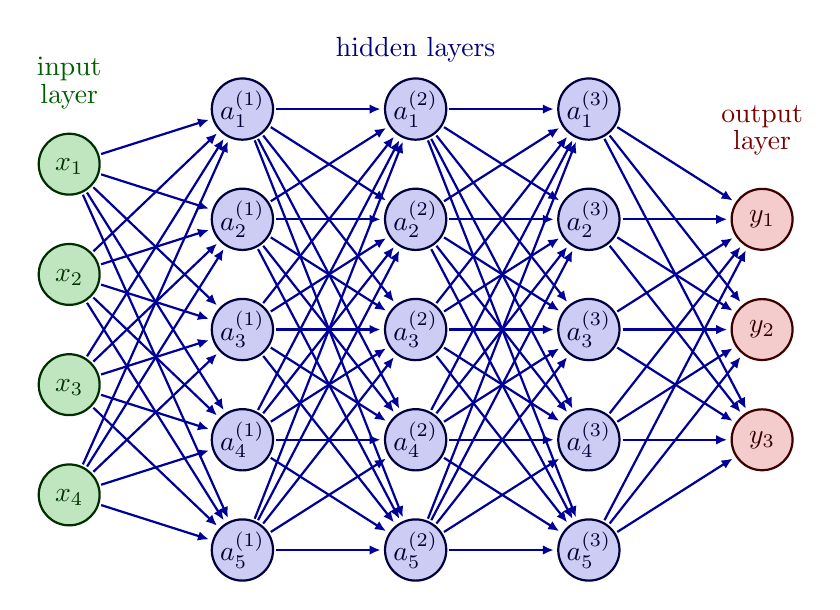
\begin{tikzpicture}[x=2.2cm,y=1.4cm]
  \message{^^JNeural network with arrows}
  \readlist\Nnod{4,5,5,5,3} % array of number of nodes per layer
  \readlist\Cstr{\strut x,a^{(\prev)},a^{(\prev)},a^{(\prev)},y} % array of coefficient symbol per layer
  
  \message{^^J  Layer}
  \foreachitem \N \in \Nnod{ % loop over layers
    \def\lay{\Ncnt} % alias of index of current layer
    \pgfmathsetmacro\prev{int(\Ncnt-1)} % number of previous layer
    \message{\lay,}
    \foreach \i [evaluate={\y=\N/2-\i; \x=\lay; \n=\nstyle;}] in {1,...,\N}{ % loop over nodes
      
      % NODES
      \node[node \n] (N\lay-\i) at (\x,\y) {$\Cstr[\lay]_{\i}$};
      %\node[circle,inner sep=2] (N\lay-\i') at (\x-0.15,\y) {}; % shifted node
      %\draw[node] (N\lay-\i) circle (\R);
      
      % CONNECTIONS
      \ifnum\lay>1 % connect to previous layer
        \foreach \j in {1,...,\Nnod[\prev]}{ % loop over nodes in previous layer
          \draw[connect arrow] (N\prev-\j) -- (N\lay-\i); % connect arrows directly
          %\draw[connect arrow] (N\prev-\j) -- (N\lay-\i'); % connect arrows to shifted node
        }
      \fi % else: nothing to connect first layer
      
    }
    
  }
  
  % LABELS
  \node[above=5,align=center,mygreen!60!black] at (N1-1.90) {input\\[-0.2em]layer};
  \node[above=2,align=center,myblue!60!black] at (N3-1.90) {hidden layers};
  \node[above=8,align=center,myred!60!black] at (N\Nnodlen-1.90) {output\\[-0.2em]layer};
  
\end{tikzpicture}




%%% LEFT NN

% NEURAL NETWORK activation
% https://www.youtube.com/watch?v=aircAruvnKk&list=PLZHQObOWTQDNU6R1_67000Dx_ZCJB-3pi&index=1
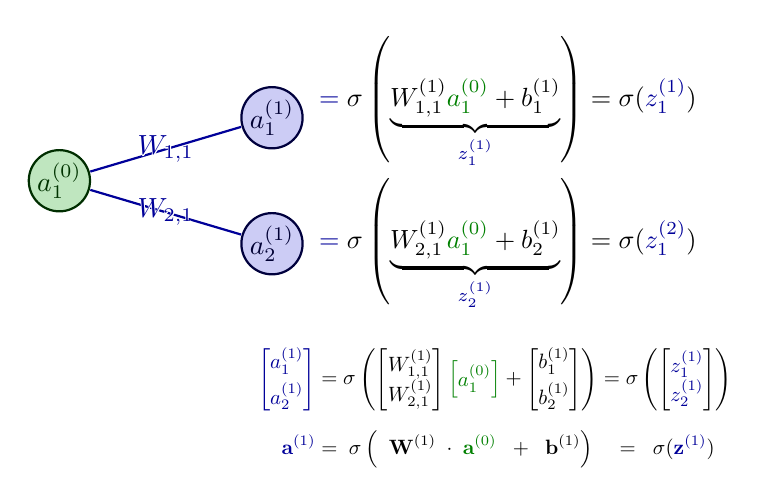
\begin{tikzpicture}[x=2.7cm,y=1.6cm]
  \message{^^JNeural network activation}
  \def\NI{1} % number of nodes in input layers
  \def\NO{2} % number of nodes in output layers
  \def\yshift{0.4} % shift last node for dots
  
  % INPUT LAYER
  \foreach \i [evaluate={\y=\NI/2-\i;}]
              in {1,...,\NI}{ % loop over nodes
    \node[node in,outer sep=0.6] (NI-\i) at (0,\y) {$a_{\i}^{(0)}$};
  }
  
  % OUTPUT LAYER
  \foreach \i [evaluate={\y=\NO/2-\i;}]
    in {\NO,...,1}{ % loop over nodes
 %   \ifnum\i=1 % high-lighted node
      \node[node hidden]
        (NO-\i) at (1,\y) {$a_{\i}^{(1)}$};
      \foreach \j  in {1,...,\NI}{ % loop over nodes in previous layer
        \draw[connect,white,line width=1.2] (NI-\j) -- (NO-\i);
        \draw[connect] (NI-\j) -- (NO-\i)
          node[pos=0.50] {\contour{white}{$W_{\i,1}$}};
      }
    % \else % other light-colored nodes
    %   \node[node,blue!20!black!80,draw=myblue!20,fill=myblue!5]
    %     (NO-\i) at (1,\y) {$a_{\i}^{(1)}$};
    %   \foreach \j in {1,...,\NI}{ % loop over nodes in previous layer
    %     %\draw[connect,white,line width=1.2] (NI-\j) -- (NO-\i);
    %     \draw[connect,myblue!20] (NI-\j) -- (NO-\i);
    %   }
    % \fi
  }
  

 % EQUATIONS
  \def\agr#1{{\color{mydarkgreen}a_{#1}^{(0)}}}
  \node[below=20,right=11,mydarkblue,scale=0.95] at (NO-1)
    {$\begin{aligned} %\underset{\text{bias}}{b_1}
       &= \color{black}\sigma\left( 
       \underbrace{\color{black}W^{(1)}_{1,1}\agr{1} + b_1^{(1)}}_{\color{mydarkblue}z^{(1)}_{1}}
             \right) = \sigma({\color{mydarkblue}z^{(1)}_{1}})\\
        &= \color{black}\sigma\left(
           \underbrace{W^{(1)}_{2,1}\agr{1} + b_2^{(1)}}_{\color{mydarkblue}z^{(1)}_{2}} 
           \color{black}\right)= \sigma({\color{mydarkblue}z^{(2)}_{1}})
      \end{aligned}$};



    
    \node[right,scale=0.75] at (0.9
    ,-2.3)
    {$\begin{aligned}
      {\color{mydarkblue}
      \begin{bmatrix}
        a_{1}^{(1)} \\[0.3em]
        a_{2}^{(1)} 
      \end{bmatrix}}
      &=
      \color{black}\sigma\left( \color{black}
      \begin{bmatrix}
        W^{(1)}_{1,1} \\
        W^{(1)}_{2,1} 
      \end{bmatrix}
      {\color{mydarkgreen}
      \begin{bmatrix}
        a_{1}^{(0)} 
      \end{bmatrix}}
      +
      \begin{bmatrix}
        b_{1}^{(1)} \\[0.3em]
        b_{2}^{(1)}
      \end{bmatrix}
      \color{black}\right)= 
      \sigma\left( 
      \begin{bmatrix}
      {\color{mydarkblue}z^{(1)}_1} \\
      {\color{mydarkblue}z^{(1)}_2}
      \end{bmatrix}
      \right)\\[0.5em] 
      {\color{mydarkblue}\mathbf{a}^{(1)}}
      &= \; \color{black}\sigma\left( \color{black}
        \;\; \mathbf{W}^{(1)} \; \cdot \; {\color{mydarkgreen}\mathbf{a}^{(0)}}
        \;\; + \;\; \mathbf{b}^{(1)}
         \color{black}\right) \quad = \;\; \sigma({\color{mydarkblue}\mathbf{z}^{(1)}})
         %\color{black},\quad \mathbf{W}^{(0)} \in \mathbb{R}^{m\times n}
    \end{aligned}$};

\end{tikzpicture}

  % RIGHT NN
  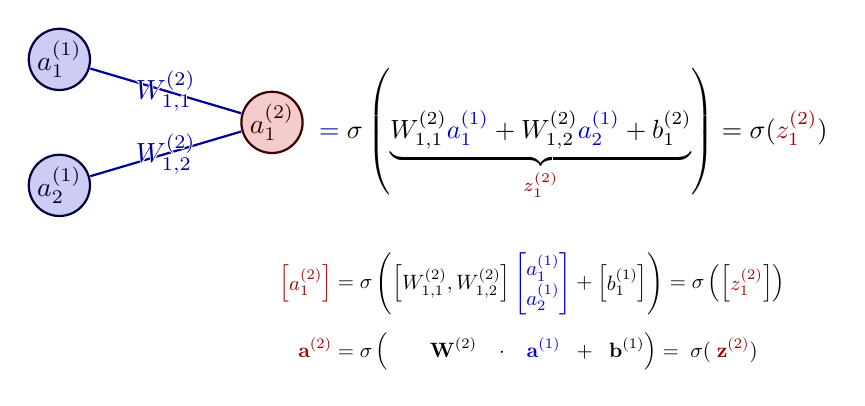
\begin{tikzpicture}[x=2.7cm,y=1.6cm]
 \message{^^JNeural network activation}
  \def\NI{2} % number of nodes in input layers
  \def\NO{1} % number of nodes in output layers
  \def\yshift{0.4} % shift last node for dots
  
  % INPUT LAYER
  \foreach \i [evaluate={\y=\NI/2-\i;}]
              in {1,...,\NI}{ % loop over nodes
    \node[node hidden,outer sep=0.6] (NI-\i) at (0,\y) {$a_{\i}^{(1)}$};
  }
  
  % OUTPUT LAYER
  \foreach \i [evaluate={\y=\NO/2-\i;}]
    in {\NO,...,1}{ % loop over nodes
 %   \ifnum\i=1 % high-lighted node
      \node[node out]
        (NO-\i) at (1,\y) {$a_{\i}^{(2)}$};
      \foreach \j  in {1,...,\NI}{ % loop over nodes in previous layer
        \draw[connect,white,line width=1.2] (NI-\j) -- (NO-\i);
        \draw[connect] (NI-\j) -- (NO-\i)
          node[pos=0.50] {\contour{white}{$W^{(2)}_{1,\j}$}};
      }
    % \else % other light-colored nodes
    %   \node[node,blue!20!black!80,draw=myblue!20,fill=myblue!5]
    %     (NO-\i) at (1,\y) {$a_{\i}^{(1)}$};
    %   \foreach \j in {1,...,\NI}{ % loop over nodes in previous layer
    %     %\draw[connect,white,line width=1.2] (NI-\j) -- (NO-\i);
    %     \draw[connect,myblue!20] (NI-\j) -- (NO-\i);
    %   }
    % \fi
  }

% EQUATIONS
  \def\agr#1{{\color{myblue}a_{#1}^{(1)}}}
  \node[below=12,right=11,mydarkblue,scale=0.95] at (NO-1)
    {$\begin{aligned} %\underset{\text{bias}}{b_1}
       &= \color{black}\sigma\left( \color{black}
            \underbrace{ W^{(2)}_{1,1}\agr{1} + W^{(2)}_{1,2}\agr{2} + b_1^{(2)}}_{{\color{mydarkred}z^{(2)}_{1}}}
             \color{black}\right) = \sigma({\color{mydarkred}z^{(2)}_{1}})\\
           \\
        %    \\
        % &= \color{mydarkred}\sigma\left( \color{black}
        %    W^{(2)}_{2,1}\agr{1} + b_2^{(2)}
        %    \color{mydarkred}\right)
      \end{aligned}$};



    
    \node[right,scale=0.75] at (1.0 ,-2.0)
    {$\begin{aligned}
      {\color{mydarkred}
      \begin{bmatrix}
        a_{1}^{(2)} 
      \end{bmatrix}}
      &=
      \color{black}\sigma\left( \color{black}
      \begin{bmatrix}
        W^{(2)}_{1,1},   W^{(2)}_{1,2} 
      \end{bmatrix}
      {\color{myblue}
      \begin{bmatrix}
        a_{1}^{(1)} \\
        a_{2}^{(1)}
      \end{bmatrix}}
      +
      \begin{bmatrix}
        b_{1}^{(1)} 
      \end{bmatrix}
      \color{black}\right)=
      \sigma\left(\begin{bmatrix}
      {\color{mydarkred}z^{(2)}_{1}}
      \end{bmatrix}
      \right)
      \\[0.5em]
      {\color{mydarkred}\mathbf{a}^{(2)}}
      &= \color{black}\sigma\left( \color{black}
           \qquad \mathbf{W}^{(2)}\;\; \; \cdot \; \;\;
           {\color{myblue}\mathbf{a}^{(1)}}
           \;\; + \;\; \mathbf{b}^{(1)}
           \color{black}\right) =
         \; \sigma( \; {\color{mydarkred}\mathbf{z}^{(2)}})
         %\color{black},\quad \mathbf{W}^{(0)} \in \mathbb{R}^{m\times n}
    \end{aligned}$};
  

\end{tikzpicture}
 \def\agr#1{{\color{mygreen}a_{#1}^{(0)}}}
 {$\begin{aligned} %\underset{\text{bias}}{b_1}
       {\color{mydarkred}\mathbf{a}^{(2)}}
       &= \color{black}\sigma\left( \color{black}
             W^{(2)}_{1,1}\color{black}\sigma\left( \color{black}
             W^{(1)}_{1,1}\agr{1} + b_1^{(1)}\right) + W^{(2)}_{1,2}\sigma\left( \color{black}
             W^{(1)}_{1,1}\agr{1} + b_1^{(1)}
             \right) + b_1^{(2)}
             \color{black}\right) =\\
           \\
      \end{aligned}$} 


\end{document}